\newpage
\section{Revisão da Teoria}

O principio de funcionamento do conversor Boost é que um indutor cria e destrói um campo magnético para resistir a mudanças bruscas de corrente. Isso permite que a tensão de saída do circuito seja maior que a tensão de entrada. Neste trabalho será analisado somente o caso em que o indutor nunca é descarregado por completo (modo contínuo).

A figura \ref{f_boost} mostra um esquemático do conversor Boost. O circuito opera em dois estados, que dependem da chave T. Estes estados são descritos abaixo.

\begin{itemize}
    \item \textbf{Chave T Fechada:} Quando a chave T está fechada (\ref{f_tclosed}), a corrente $I_L$ flui através do indutor L, no sentido horário. Isso faz com que o indutor armazene energia na forma de campo magnético. Enquanto o interruptor carrega, uma tensão $V_l$ aparece sobre o mesmo, tendo como lado positivo o lado esquerdo.
    
    \item \textbf{Chave T Aberta:} Ao abrir a chave, a corrente $I_L$ que passava no indutor se manterá (não há variação de corrente instantânea no indutor), porém a tensão em cima do mesmo será diferente, dado que a impedância vista pelo indutor mudou. Para manter a corrente, o campo magnético que havia sido criado previamente, será agora destruído. Isso fará com que a polaridade da tensão em cima do indutor ($V_L$) mude de sentido. Do ponto de vista da carga, agora são duas fontes de tensão em série, como indicado na figura \ref{f_opened}.
\end{itemize}


\begin{figure}[H]
    \centering
    \caption{Esquemático do conversor Boost.}
    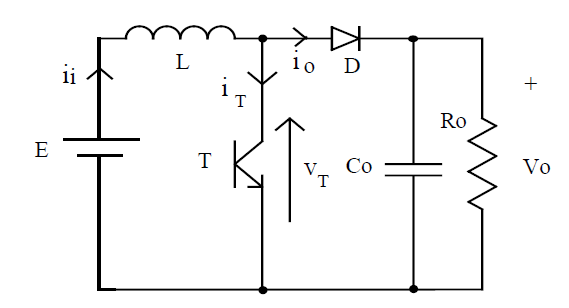
\includegraphics[scale = 0.5]{boost}
    \label{f_boost}
\end{figure}

Vale notar que, para que o conversor opere no modo contínuo, a frequência de chaveamento deve ser alta o suficiente para manter uma carga mínima no indutor.

Um característica importante do conversor Boost é que a corrente de entrada é constante, ou seja, há pouco ruído indo para a fonte de alimentação.

\subsection{Ganho estático}

    Para os cálculos do ganho de tensão no conversor Boost, vamos considerar os componentes ideais, o circuito no regime estático de operação e que a corrente no indutor nunca chega a zero (modo contínuo).
    
    Quando a chave está fechada (figura \ref{f_tclosed}), aparece uma tensão $V_i$ em cima do indutor, a qual causa uma corrente $I_L$ através do indutor durante um período de tempo $\tau$. A corrente e a tensão no indutor estão relacionadas pela equação geral do indutor (\ref{e_Vl}).
    
    \begin{equation}
        V_L = L\frac{\Delta I_L}{\Delta t}
        \label{e_Vl}
    \end{equation}

    Ao final do período $\tau$, a corrente $I_L$ é
    
    \begin{equation}
        \Delta I_{L_{On}}=\frac{1}{L}\int_0^{D T}V_i d t=\frac{D T}{L} V_i.
        \label{e_ilon}
    \end{equation}
    
    Onde D é a razão cíclica (fração do período T no qual a chave T fica fechada).

    \begin{figure}[H]
        \centering
        \caption{Conversor Boost com a chave T fechada.}
        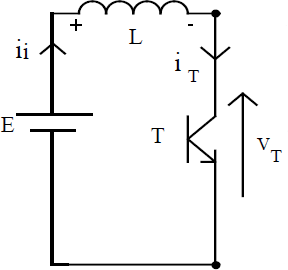
\includegraphics[scale = 0.5]{tclosed}
        \label{f_tclosed}
    \end{figure}

    Ao abrir a chave (figura \ref{f_opened}), a corrente que passa através do diodo fluirá através da carga. Porém, conforme a energia no indutor é transferida para a carga, a tensão no indutor diminui. Assim, a tensão $V_L$ será

    \[
        V_L = V_i-V_o = L\frac{dI_L}{dt}.
    \]

    Então, a variação de $I_L$ se da por

    
    \begin{equation}
        \Delta I_{L_{Off}}=\int_{DT}^{T}\frac{\left(V_i-V_o\right) dt}{L}=\frac{\left(V_i-V_o\right) \left(1-D\right) T}{L}.
        \label{e_iloff}
    \end{equation}
    

\begin{figure}[H]
    \centering
    \caption{Conversor Boost com a chave T aberta.}
    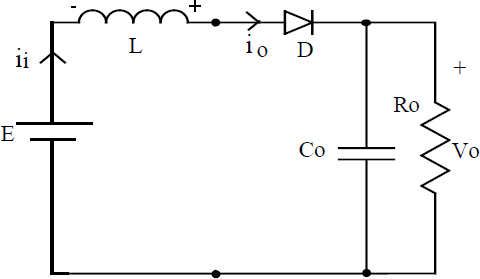
\includegraphics[scale = 0.5]{topened}
    \label{f_opened}
\end{figure}

    Para que o indutor não sature, é necessário que a energia armazena durante o período de carregamento seja liberada durante o período de descarregamento do indutor. Ou seja

    
    \begin{equation}
        \Delta I_{L_{On}} + \Delta I_{L_{Off}}=0.
        \label{e_dilzero}
    \end{equation}
    
    
    Substituindo \ref{e_ilon} e \ref{e_iloff} em \ref{e_dilzero}, temos que
    
    \[
        \Delta I_{L_{On}} + \Delta I_{L_{Off}}=\frac{V_i D T}{L}+\frac{\left(V_i-V_o\right)\left(1-D\right)T}{L}=0.
    \]

    A qual pode ser reescrita como
    
    \begin{equation}
        \frac{V_o}{V_i}=\frac{1}{1-D}.
        \label{e_ganho}
    \end{equation}
    
    Esta é a equação do ganho estático para o conversor Boost em modo contínuo. Observe que a tensão de saída será sempre maior ou igual a tensão de entrada e que, teoricamente, a tensão de saída sobe até o infinito conforme D se aproxima de 1.